\documentclass[colorthm]{./civarticle}
\usepackage{graphicx} % Required for inserting images
\usepackage[math]{blindtext}
\usepackage{float}

\title{Цифровые подписи}
\author{Захар Назаров}
\date{Июнь 2024}

\begin{document}

\section{Введение}
Что-то

\section{Термины и определения}

\begin{definition}
    \textbf{Схема "Hash-and-Sign"}

    Пусть $\Pi = (\text{Gen}, \text{Sign}, \text{Vrfy})$ — это схема подписи для сообщений длиной $l(n)$, и пусть $\Pi_H = (\text{Gen}_H, H)$ — это хеш-функция с выходной длиной $l(n)$. Построим схему подписи $\Pi' = (\text{Gen'}, \text{Sign'}, \text{Vrfy'})$ следующим образом:
    \begin{itemize}
        \item $\text{Gen'}$: на вход $1^n$ запускаем $\text{Gen}(1^n)$, чтобы получить $(pk, sk)$, и запускаем $\text{Gen}_H(1^n)$, чтобы получить $s$; открытый ключ равен $\langle pk, s \rangle$, а закрытый ключ равен $\langle sk, s \rangle$.
        
        \item $\text{Sign'}$: на вход подается закрытый ключ $\langle sk, s \rangle$ и сообщение $m \in \{0, 1\}^*$, на выходе $\sigma \leftarrow \text{Sign}_{sk}(H_s(m))$.
        
        \item $\text{Vrfy'}$: на вход подается открытый ключ $\langle pk, s \rangle$, сообщение $m \in \{0, 1\}^*$ и подпись $\sigma$, на выходе выдать 1, если и только если $\text{Vrfy}_{pk}(H_s(m), \sigma) \stackrel{?}{=} 1$.
    \end{itemize}

    Построенная $\Pi'$ и будет схемой подписи "Hash-and-Sign".
\end{definition}

\begin{definition}
    Эллиптической кривой над конечным полем $F_q$ называется совокупность точек $(x, y)$, которые удовлетворяют следующему уравнению:

    $y^2 = x^3 + ax + b$

    Над точками эллиптической кривой вводится операция сложения с помощью добавления "виртуальной точки" O. Лучше всего варианты сложения точек эллиптической кривой описываются следующей иллюстрацией:

    \begin{figure}[H]
        \centering
        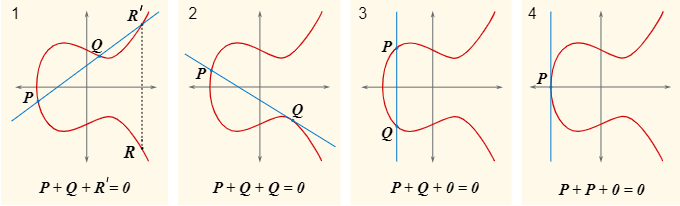
\includegraphics[width=0.75\linewidth]{ECClines-2.0.png}
        \caption{Операция сложения для точек эллиптической кривой [4]}
        \label{fig:enter-label}
    \end{figure}

    Умножение точки на целое число $Q=nP$ определяется как:
    \begin{displaymath}Q = \sum_{n} P\end{displaymath}.

\end{definition}

\begin{definition}
    Дерево Меркла?
\end{definition}


\section{Архитектуры хеш-функций}
Рассмотрим две основные архитектуры построения схем подписей: "Hash-and-Sign" и "преобразование Фиата–Шамира"

\subsection{Hash-and-Sign}

Пусть у нас есть схема подписи $\Pi$ сообщений длины $l$ и хеш-функция $H$, у которой длина выхода также равна $l$. Схема "Hash-and-Sign" заключается в том, что сообщение произвольной длины хеширутеся с помощью $H$ и затем подписывается $\Pi$.

Формальное определение содержится в главе "Термины и определение".


\subsection{Преобразование Фиата–Шамира}

В 1986 году Амос Фиат и Ади Шамир опубликовали новый протокол интерактивного взаимодействия, с помощью которого можно организовать идентификацию и  схемы подписи [1]. Его криптографическая стойкость основана на сложности решения задачи нахождения квадратного корня из числа по модулю $n$, где $n$ - это произведение двух простых чисел и двоичная запись $n$ содержит не менее 512 значащих битов. Также классическая схема предполагает наличие \textbf{доверенного} центра, который будет подтверждать информацию $I$ об идентифицирующейся стороне и выдавать ей определенный секрет под эти данные. 
Зафиксируем:

\begin{enumerate}
    \item Публичное число $n=pq$, где $p,q$ - простые числа. Факторизацию этого числа знает только доверенный центр.
    \item Публичная псевдослучайная функция $f$.
    \item Фиксированное количество $k$ маленьких значений $j$. Для простоты зафиксируем: $j = 1, \ldots, k$.
    \item Количество проверок $t$.
\end{enumerate}

Поэтому эта схема содержит 2 этапа: проверка идентичности доверенным центром и выдача секрета идентифицирующейся стороне, непосредственная идентификация перед контрагентом.

\textbf{Этап проверки идентичности}

\begin{enumerate}
    \item Центр вычисляет $k$ значений $v_j = f(I, j)$.
    \item Для каждого $v_j$ находится обратный к нему элемент $p = v^{-1}_j$ по модулю $n$ и затем вычисляется наименьший квадратный корень по модулю: $s_j = \sqrt{p}$ mod $n$.
    \item Затем безопасным путем (в оригинальной статье в виде смарт-карты) передается информация идентифицирующейся стороне: $I, s_j (и соответствующие индексы j)$. 
\end{enumerate}

\textbf{Идентификация}

Пусть у нас есть A со смарт-картой и сторона B, перед которой A хочет идентифицироваться.

\begin{enumerate}
    \item Сторона A отправляет I стороне B.
    \item B вычисляет $v_j = f(I, j)$, где $j=1,\ldots, k$.
    \item Для i от 1 до t:

        \begin{enumerate}
            \item Сторона A выбирает случайное $r_i \in [0, n)$ и отправляет $x_i=r^{2}_{i}$ стороне B.
            \item Сторона B отправляет рандомный бинарный вектор $(e_{i1}, \ldots, e_{ik})$ стороне А.
            \item Сторона A отправляет B:

            $y_i=r_i \prod_{e_{i j}=1} s_j \quad(\bmod n)$

            \item Сторона B проверяет:

            $x_i = y^{2}_{i} \prod_{e_{i j}=1} v_j \quad(\bmod n)$ 
        \end{enumerate}
    
\end{enumerate}

Таким образом, если все проверки B прошли успешно, то считается что A успешно идентифицировалась. В противном случае - не успешно.


\section{DSA}
DSA (Digital Signature Algorithm) - алгоритм цифровой подписи, основанный на конструкции "Hash-and-sign". Опубликован в 1998 году и запатентован NIST. Опишем алгоритм, следуя стандарту [2].

Определим следующие параметры:

\begin{enumerate}
    \item Простое число $p$, где $2^{L-1} < p < 2^{L}$, $512<=L<=1024$ и $L$ кратно 64.
    \item Простое число $q$, которое является делителем $p-1$, $2^{159} < q < 2^{160}$.
    \item $g=h^{(p-1)/q}$ mod $p$, где $h$ любое число от $1$ до $p-1$ и $g > 1$.
    \item Случайное число $x$, сгенерированное псевдорандомно, $0 < x < q$. 
    \item $y = g^x$ mod $p$
    \item Случайное число $k$, сгенерированное псевдорандомно, $0 < k < q$. 
\end{enumerate}

Значения p, q, g публичны и ими может пользоваться группа пользователей. Приватный и публичный ключ пользователя x и y соответственно. Значения x и k используются для генерации подписи и остаются в секрете, k генерируется для каждой новой подписи. 

\subsection{Генерация цифровой подписи}

\begin{enumerate}
    \item $r = (g^k $ mod $ p) $ mod $ q$
    \item $(k^{-1}()SHA-1(M) + xr) $ mod $ q$
\end{enumerate}

Значение $k^{-1}$ является мультипликативно обратным элементом к $k$ по модулю q. Если $r=0$, то выбирается другое $k$; если $s=0$, то выбирается другое $k$. Далее сообщение $m$ отправляется вместе с подписью $(r, S)$ получателю.

\subsection{Проверка цифровой подписи}

Получатель знает $p, q, g, y$ и получает подписанное сообщение $(m, r, s)$. Алгоритм проверки следующий:

\begin{enumerate}
    \item Проверяется что r,s лежат в диапазоне: $0 < r, s < q$. Иначе проверка заканчивается неуспехом. Если все правильно, то проводятся дальнейшие вычисления.
    \item $w = s^{-1} $ mod $ q$
    \item $u_1 = ((SHA-1(M))w) $ mod $ q$
    \item $u_2 = ((r)w) $ mod $ q$
    \item $v = (((g)^{u_1}(y)^{u_2}) $ mod $ p) $ mod $ q$
\end{enumerate}

Если $v=r$, то подпись считается валидно, иначе - невалидной.


\section{ECDSA}
ECDSA (Elliptic Curve Digital Signature Algorithm) - алгоритм цифровой подписи, основанный на конструкции "Hash-and-sign", а также использующий эллиптические кривые.

Будем считать, что у нас есть заданная эллиптическая кривая с параметрами, которая отвечает требованиям безопасности, описанным в стандарте [3]:

\begin{enumerate}
    \item $q$ - порядок поля $F_q$.
    \item $n$ - порядок эллиптической кривой.
    \item $a, b$ - параметры эллиптической кривой.
    \item $G$ - базовая точка эллиптической кривой.
\end{enumerate}

Начнем рассматривать взаимодействие между A и B, где A - хочет отправить подписанное сообщение.

\subsection{Генерация ключевой пары}
На входе у нас заданная эллиптическая кривая и точка $G$.

\begin{enumerate}
    \item Выбирается случайное число $d \in [1, n-1]$.
    \item Вычисляется новая точка эллиптической кривой $Q=dG$.
    \item На выход идет $d$ и $Q$.
\end{enumerate}

\subsection{Генерация цифровой подписи}
На входе у нас заданная эллиптическая кривая, точка $G$, закрытый ключ $d$, хеш-функция $H$ и сообщение $m$.

\begin{enumerate}
    \item Выбирается случайное число $k \in [1, n-1]$.
    \item Вычислить $kG = (x_1, y_1)$.
    \item Вычислить $r = x_1$ mod $n$.
    \item Вычислить $e = H(m)$
    \item Вычислить $s = k^{-1}(e+dr)$ mod $n$
    \item Вернуть $(r, s)$
\end{enumerate}

Если $r=0$, то выбирается другое $k$; если $s=0$, то выбирается другое $k$.

\subsection{Проверка цифровой подписи}
На входе у нас заданная эллиптическая кривая, точка $G$, хеш-функция $H$, сообщение $m$, открытый ключ $Q$ и подпись $(r, s)$.

\begin{enumerate}
    \item Проверка, что $r, s \in [1, n-1]$. При неудаче - то подпись невалидна.
    \item Вычислить $e = H(m)$.
    \item Вычислить $w = s^{-1} $ mod $n$.
    \item Вычислить $u_1 = ew$ mod $n$, $u_2 = rw$ mod $n$.
    \item Вычислить $X = u_1*G + u_2*Q = (x_2, y_2)$
    \item Если $X = O$, то подпись невалидна. Иначе вычислить $v = x_2 $ mod $ n$
\end{enumerate}

Если $v = r$, то подпись валидна, иначе - невалидна.

\section{ГОСТ Р 34.10-1994}
ГОСТ Р 34.10-1994 - алгоритм цифровой подписи, основанный на конструкции "Hash-and-sign", стандартизованный в 1994 году [5].

Пусть заданы простые числа $p$ (512 бит) и $q$ (256 бит), которые удовлетворяют условиям описанным в стандарте [5]. Пусть также есть число $a > 1$, которое представляется в виде:

$a = d^{\frac{p-1}{q}}$ mod $p$ (512 бит)

\subsection{Генерация цифровой подписи}
На входе у нас заданные $p, q, a$, сообщение $m$ и хеш-функция $H$. Предварительно выбирается случайное число $x \in [0, q]$, которое будет закрытым ключом. Также считается открытый ключ по формуле: $y = a^x$ mod $p$.

\begin{enumerate}
    \item Вычислить $h=H(m)$ mod $q$, если $H(M)=0$, то $h:=0^{255}1$.
    \item Выбирается случайное число $k \in [0, q]$.
    \item Вычислить $r = a^k$ mod $p$.
    \item Вычислить $r' = r$ mod $q$.
    \item Если $r'=0$, то выбрать другое $k$.
    \item Вычислить $s = (xr'+kh)$ mod $q$.
    \item Подать на выход подпись: $(r', s)$
\end{enumerate}

После выработки подписи число $k$ уничтожается.

\subsection{Проверка цифровой подписи}
На входе у нас заданные $p, q, a$, сообщение $m$, хеш-функция $H$, открытый ключ $y$ и подпись $(r', s)$.

\begin{enumerate}
    \item Проверка, что $r', s \in (0, q)$. При неудаче - то подпись невалидна.
    \item Вычислить $h=H(m)$ mod $q$, если $H(M)=0$, то $h:=0^{255}1$.
    \item Вычислить $v=h^{q-2}$ mod $q$.
    \item Вычислить $z_1=sv$ mod $q$.
    \item Вычислить $z_2=(q-r')v$ mod $q$.
    \item Вычислить $u=((a^{z_1}*y^{z_2})$ mod $p)$ mod $q$.
    \item 
\end{enumerate}

Если $u = r'$, то подпись валидна, иначе - невалидна.

\section{ГОСТ 34.10-2018}
ГОСТ Р 34.10-2018 - алгоритм цифровой подписи, основанный на конструкции "Hash-and-sign", а также использующий эллиптические кривые. Является международным стандартом, принятым в 2018 году [6].

Будем считать, что у нас есть заданная эллиптическая кривая с параметрами, которая отвечает требованиям безопасности, описанным в стандарте [6]:

\begin{enumerate}
    \item $p$ - порядок поля $F_p$.
    \item $m$ - порядок эллиптической кривой.
    \item $a, b$ - параметры эллиптической кривой.
    \item $P$ - базовая точка эллиптической кривой.
    \item $H(M)$ - хеш-функция (ГОСТ Р 34.11-2012 [Стрибог]), с выходом 256-бит.
\end{enumerate}

Начнем рассматривать взаимодействие между A и B, где A - хочет отправить подписанное сообщение.

\subsection{Генерация ключевой пары}

\begin{enumerate}
    \item Выбирается случайное число $d \in [1, q-1]$.
    \item Вычисляется новая точка эллиптической кривой $Q=dP$.
    \item На выход идет $d$ и $Q$.
\end{enumerate}

\subsection{Генерация цифровой подписи}
На входе у нас заданная эллиптическая кривая, закрытый ключ $d$, и сообщение $m$.

\begin{enumerate}
    \item Вычислить $h = H(m)$
    \item Вычислить $e = h$ mod $q$. Если $e=0$, то $e$ := $1$
    \item Выбирается случайное число $k \in [1, q-1]$.
    \item Вычислить $C=kP = (x_1, y_1)$.
    \item Вычислить $r = x_1$ mod $q$.
    \item Вычислить $s = (rd + ke)$ mod $q$
    \item Вернуть $(r, s)$
\end{enumerate}

Если $r=0$, то выбирается другое $k$; если $s=0$, то выбирается другое $k$.

\subsection{Проверка цифровой подписи}
На входе у нас заданная эллиптическая кривая, сообщение $m$, открытый ключ $Q$ и подпись $(r, s)$.

\begin{enumerate}
    \item Проверка, что $r, s \in [1, q-1]$. При неудаче - то подпись невалидна.
    \item Вычислить $h = H(m)$.
    \item Вычислить $e = h$ mod $q$. Если $e=0$, то $e$ := $1$
    \item Вычислить $v = e^{-1} $ mod $q$.
    \item Вычислить $z_1 = sv$ mod $q$, $z_2 = -rv$ mod $q$.
    \item Вычислить $C = z_1*P + z_2*Q = (x_2, y_2)$
    \item Вычислить $R = x_2 $ mod $q$
\end{enumerate}

Если $R = r$, то подпись валидна, иначе - невалидна.

\section{Схема подписи Фиата–Шамира}
Схема подписи Фиата–Шамира получается из преобразования Фиата–Шамира с помощью модификации. 

Пусть A хочет отправить подписанное сообщение M стороне B. 

\begin{itemize}
    \item В данном случае теперь у нас нет доверенного центра, сторона А сама определяет число $n=pq$.
    \item Затем A генерирует секретную последовательность из z чисел $x_0, \ldots, x_z$ таких, что: $n $ div $ 2^{64} <=x_i<= n-1$ и $GCD(x_i, n) = 1$, где $GCD(a, b)$ - наибольший общий делитель a и b.
    \item Далее A генерирует публичную последовательность $y_0, \ldots, y_z$, которая вычисляется по формуле:

    $y_i = x^{-2}_i$ mod $n$.
\end{itemize}

Пусть A хочет отправить сообщение M стороне B. Пусть у нас также задана хеш-функция $H$.

\subsection{Процесс взаимодействия сторон}

\begin{enumerate}
    \item Сторона A выбирает случайное $k \in [0, n)$ и отправляет $R=k^{2}$ стороне B. 
    \item Сторона B отправляет рандомный бинарный вектор $(e_{i1}, \ldots, e_{iz})$ стороне А.
    \item Сторона А вычисляет хеш $E=H(M||R)$.
    \item Сторона A вычисляет: $S=k \prod_{e_{ij}=1} x_i \quad(\bmod n)$.
    \item Сторона A отправляет $(M, E, S)$ стороне B.
    \item Сторона B вычисляет: $R' = S^{2} \prod_{e_{ij}=1} y_j \quad(\bmod n)$
    \item Сторона B вычисляет: $E'=H(M||R')$.
    \item Если $E=E'$, то подпись валидна, иначе - невалидна.
\end{enumerate}

Отметим, что сторона B знает публичную последовательность $y_0, \ldots, y_z$ стороны A (аналог публичного ключа). Также интересно, что для одного и того же сообщения для разных посылок, будут разные подписи из-за генерации $k$.

\section{Схема подписи Шнорра}
Схема подписи Шнорра - схема подписи, которая является модификацией схемы подписи Фиата-Шамира.

\subsection{Генерация ключей}

\begin{enumerate}
    \item Сторона А выбирает простоe число $p$ длиной 1024 бит.
    \item Сторона А выбирает простоe число $q$, такое что оно является делителем числа $p-1$. Размер $q$ равен 160 бит.
    \item Сторона А выбирает $g > 1$, такое что $g^q=1$ mod $p$.
    \item Сторона А выбирает случайное число $w < q$.
    \item Сторона А вычисляет $y = g^{q-w}$ mod $p$.
\end{enumerate}

Таким образом у A появляется открытый ключ $(p, q, g, y)$ и секретный ключ $w$.

Пусть A хочет отправить сообщение M стороне B. Пусть у нас также задана хеш-функция $H$.

\subsection{Генерация цифровой подписи}

\begin{enumerate}
    \item Сторона А выбирает случайное число $r < q$ и вычисляет $x = g^r$ mod $p$.
    \item Сторона А вычисляет $S_1=H(M||x)$.
    \item Сторона A вычисляет $S_2=r+wS_1$ mod $q$.
    \item Сторона А отправляет стороне B подписанное сообщение $(M, S_1, S_2)$.
\end{enumerate}

\subsection{Проверка цифровой подписи}

\begin{enumerate}
    \item Сторона B вычисляет $X=(g^{S_2}g^{S_1}) $ mod $p$.
    \item Сторона B вычисляет $S'=H(M||X)$
\end{enumerate}

Если $S' = S_1$, то подпись валидна, иначе - невалидна.

\section{Схема подписи Меркля–Лампорта}
Схема подписи Меркля–Лампорта - это схема цифровой подписи, основанная на использовании дерева Меркла и на одноразовой цифровой подписи Лампарта [7].

\subsection{Цифровая подпись Лампарта}

Пусть A хочет отправить сообщение $M$ стороне B. Пусть задано положительное число $k$, $M \in \{0, 1\}^k$. Пусть у нас также задана хеш-функция $H$. 

\subsubsection{Генерация ключей}

Генерируется $2r$ значений $y_{ij}$, где $1<=i<=k$, $0<=j<=1$. Также вычисляется для всех $i,j$ : $z_{ij}$ = $H(y_{ij})$.

Набор $y_{ij}$ - это закрытый ключ.
Набор $z_{ij}$ - это открытый ключ.

\subsubsection{Генерация цифровой подписи}

Пусть $M=m_1||m_2||\ldots||m_k$.
Подпись сообщения $sign$ считается как: $sign=(y_{1, m_1}, \ldots, y_{k, m_k})=(s_1, \ldots, s_k)$

\subsubsection{Проверка цифровой подписи}

Если для всех $1<=i<=k$ верно: $f(s_i) = z_{i, m_i}$, то подпись $sign$ считается валидной, иначе - невалидной.

\subsection{Подпись Лампарта в комбинации с деревом Меркла}

В подписи Лампарта открытый ключ может использоваться только 1 раз. С помощью дерева Меркла можно создать схему подписи, где открытый ключ может использоваться несколько раз (при большом дереве, можно считать, что ключ можно использовать неограниченное количество раз).

\subsubsection{Генерация ключей}

Зададим некоторое $n > 1$. Сгенерируем $2^n$ пар ключей Лампарта $(X_i, Y_i)$ ($1<=i<=2^n)$, где $X_i$ - закрытый ключ, $Y_i$ - открытый ключ.

Затем посчитаем для каждого открытого ключа посчитаем его хеш: $h_i = H(Y_i)$, $1<=i<=2^n$.

Построим дерево Меркла с листьями $(h_1, \ldots, h_{2^n})$. Пусть корень дерева $pub$ будет открытым ключом для новой схемы подписи.

\subsubsection{Генерация цифровой подписи}

Выберем любую пару ключей $X_i, Y_i$, например $X_d, Y_d$. Подпишем ею сообщение $M$, получим подпись $sig'$. Возьмем хеш от публичного ключа $h_d = H(Y_d)$. В дереве Меркла это будет лист. Встанем на этот лист и возьмем соседний элемент (назовем его $a_0$), который тоже ведет к родителю $h_d$. Встанем теперь на родителя $h_d$ и также возьмем элемент (назовем его $a_1$), который ведет к родителю родителя $h_d$. И так далее, пока не дойдем до вершины. Последний взятый элемент $a_{n-1}$ будет иметь родителя $pub$.

Составим итоговую подпись сообщения $M$ в новой схеме: 

$sig=(siq', Y_d, a_0, \ldots, a_{n-1})$

\subsubsection{Проверка цифровой подписи}

Сначала проверяется одноразовая подпись $sig'$. Если она валидна, то идем дальше, если нет - $sig$ также считается невалидной. Если $sig'$ валидна, то считаем $A_0 = H(Y_d)$. Затем считаем $A_i = H(A_{i-1}||a_i)$ для $0<=i<=n-1$.

Если $A_{n-1} = pub$, то подпись валидна, иначе - невалидна.

\section{Схема подписи CFS(Courtois, Finiasz, Sendrier)}
Схема подписи CFS(Courtois, Finiasz, Sendrier) - алгоритм цифровой подписи, основанный на конструкции "Hash-and-sign", а также использующий линейные коды. Этот алгоритм был предложен в 2001 году [8] исследователями Courtois, Finiasz и Sendrier.

Ее безопасность опирается на сложность декодирования, а также на сложность восстановления структуры линейного кода.

Пусть A хочет отправить сообщение $M$ стороне B. 

Зафиксируем:

\begin{itemize}
    \item Пусть заданы целые числа $n,k$, которые определяют размерность линейного кода $C[n, k]$.
    \item Пусть у нас задана хеш-функция $H$ с выходом размера $n-k$.
    \item Пусть у нас задана случайная бинарная невырожденная квадратная матрица $S$ порядка $(n-k)$ .
    \item Пусть у нас задана случайная бинарная матрица перестановки $P$ порядка $n$.
\end{itemize} 

Будем считать, что вышеописанные параметры отвечают требованиями безопасности, описанным в [8].
 
\subsubsection{Генерация ключей}

Секретным ключом является линейный код $C_0[n, k]$ с генератором $G_0$ и матрицей проверки $H_0$.

Публичным ключом является: $H=V*H_0*P$.

\subsubsection{Генерация цифровой подписи}

\begin{enumerate}
    \item Вычисляется хеш $s=H(M)$.
    \item Вычисляются $s_i=h(s||i)$, $i=0,1,2,\ldots$, до тех пор пока какое-то $s_{i_0}$ не станет декодируемым для $C_0$. Запомним этот $s_{i_0}$.
    \item Затем с помощью обратной функции(trapdoor function) мы находим такое $z$, что $H*z^T=s_{i_0}$.
    \item На выход идет подпись $(z, i_0)$.
\end{enumerate}$

\subsubsection{Проверка цифровой подписи}

\begin{enumerate}
    \item Вычисляется хеш $s=H(M)$.
    \item Вычислить $s_1 = H*z^T$
    \item Вычислить $s_2=h(s||i_0)$
\end{enumerate}

Если $s_1 = s_2$, то подпись валидна, иначе - нет. Для оптимизации разработчики преобразуют $z$, чтобы подпись была более компактная.

\subsection{Криптоанализ}
Как говорилось выше, безопасность этой схемы опирается на сложность декодирования, а также на сложность восстановления структуры линейного кода. Поэтому рассмотрим атаки именно на эти аспекты.

\subsubsection{Декодирующие атаки}
Наиболее известная атака методом декодирования была предложена Каньто и Шабо [10], и её асимптотическая временная сложность составляет примерно $(n/log_2(n))^{f(t)}$, где $f(t)=\lambda * t - c$ является аффинной функцией с $\lambda$, не сильно меньшим единицы, и $c$ — константой, лежащей в пределах от 1 до 2.

Хорошие оценки асимптотического поведения сложности лучших известных общих методов декодирования приведены Баргом в [11]. В действительности, когда скорость $(R = \frac{k}{n}$ кода стремится к 1, временная и объем памяти становится $(2^{n(1-R)/2(1+o(1))})$, что для кодов Гоппа даёт $(n^{t(1/2+o(1))})$.

\subsubsection{Структурные атаки}
Немного известно о различимости кодов Гоппы. На практике единственная структурная атака [12] заключается в перечислении всех кодов Гоппы и затем тестировании их на эквивалентность с открытым ключом. Существует $(2^{tm}/t)$ бинарных кодов Гоппы, исправляющих t ошибок, длины $(n = 2^m)$, но из-за свойств кодов Гоппа нужно проверить только один из $(mn^3)$, и, наконец, сложность проверки эквивалентности не может быть ниже $(n(tm)^2)$ (методом Гауссова исключения). В итоге, совокупная сложность структурной атаки не будет меньше чем $(tmn^{t-2})$ элементарных операций.

\subsubsection{Сложность}
Пусть $n=2^m$, $k=n-tm, d>=2t+1$ для кода Гоппа. Тогда сложность лучших атак будет:

\begin{itemize}
    \item Для декодирующей атаки: $2^{t m(1 / 2+o(1))}$
    \item Для структурной атаки: $\operatorname{tm} 2^{m(t-2)}$
\end{itemize}

\subsection{Заключение}
**Вывод:**

Схема цифровой подписи CFS (Courtois, Finiasz, Sendrier) основана на методе "Hash-and-sign" и использует линейные коды для обеспечения безопасности. Безопасность данной схемы зависит от сложности декодирования и восстановления структуры линейного кода, что делает её устойчивой к широкому спектру атак. Основные атаки для схемы это декодирующие и структурные атаки. Временная и пространственная сложность этих атак варьируется в зависимости от параметров кода, однако лучшие известные атаки всё ещё имеют достаточно высокую вычислительную сложность.

\section{CRYSTALS–Dilithium. My Signature!}
CRYSTALS–Dilithium - постквантовый алгоритм цифровой подписи, опубликованный в 2021 году [9].

\subsubsection{Генерация ключей}

\begin{itemize}
    \item Генерация матрицы A размера $k*l$, элементами которой являются полиномы в кольце $R_q=Z_q[n]/(X^n+1)$. Эта матрица - первая часть публичного ключа.
    \item Генерация двух случайных векторов $(s_1, s_2)$ размеров l и k соответственно. Элементом вектора являются также полиномы в кольце $R_q$ (с коэффициентами у многочленов не больше $\eta$.
    \item Вычислить $t=A*s_1+s_2$.
\end{itemize}

Таким образом,

Пара (A, t) - публичный ключ.

Пара (A, t, $s_1$, $s_2$) - приватный ключ.

$\newline$

Пусть A хочет отправить сообщение M стороне B. Пусть у нас также задана хеш-функция $H$.

Определим вспомогательные функции:

\begin{figure}[H]
    \centering
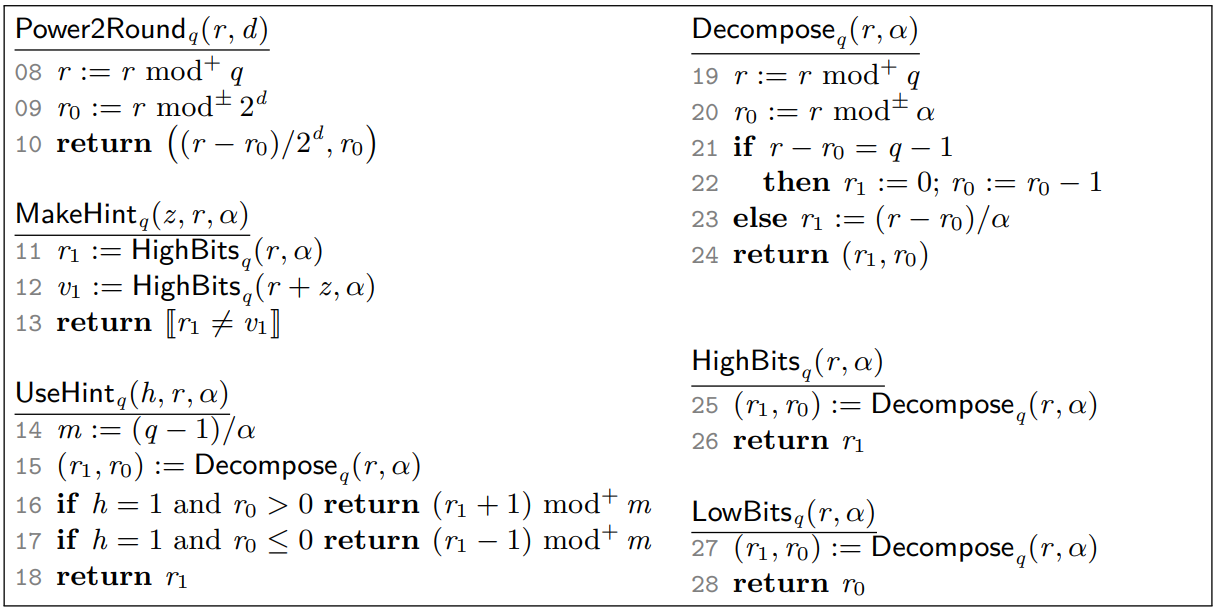
\includegraphics[width=0.5\linewidth]{crytst_func.png}
    \caption{Вспомогательные функции для CRYSTALS–Dilithium [9].}
    \label{fig:enter-label}
\end{figure}

\subsubsection{Генерация цифровой подписи}

\begin{enumerate}
    \item Генерация вектора-маски $y \in S^{l}_{\upgamma_1 - 1}$, который состоит из многочленов с коэффициентами меньше, чем $\upgamma_1$. Считаем, что $\upgamma_1$ отвечает требованиям безопасности, описанным в [9].
    \item  Вычисляем $w_1=HighBits(Ay, 2*\upgamma_2)$. Считаем, что $\upgamma_2$ отвечает требованиям безопасности, описанным в [9].
    \item Вычислить $c=H(M||w_1)$, $c \in B_{60}$. $c$ - это многочлен в $R_q$, имеющий ровно 60 коэффициентов, которые равны 1 или -1, остальные - нули.
    \item $\beta = max(c*s_1, c*s_2)$
    \item Если один из коэффициентов z, больше чем $\upgamma_1 - \beta$, то генерация подписи начинается заново. 
    \item Если все коэффициенты младших битов $Az - ct$, больше чем $\upgamma_2 - \beta$, то генерация подписи начинается заново. 
    \item На выход идет подпись $(z, c)$.
\end{enumerate}

\subsubsection{Проверка цифровой подписи}

\begin{enumerate}
    \item Вычислить $w'_1=HighBits(Az-ct, 2\upgamma_2$.
    \item Если один из коэффициентов z, больше чем $\upgamma_1 - \beta$, то подпись невалидна. 
    \item Вычислить $c'=H(M||w'_1)$ 
\end{enumerate}

Если с' = с, то подпись валидна, иначе - нет.

\subsubsection{Листинг полного алгоритма}

\begin{figure}[H]
    \centering
    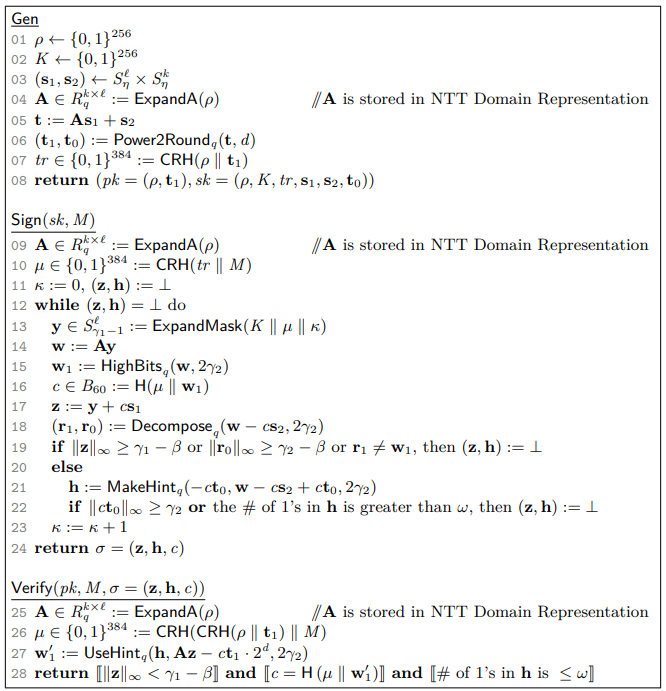
\includegraphics[width=0.5\linewidth]{cryst_list.png}
    \caption{Листинг CRYSTALS–Dilithium [9]}
    \label{fig:enter-label}
\end{figure}

\section{Список литературы}
[1] Fiat A., Shamir A. How to prove yourself: Practical solutions to identification and signature problems //Conference on the theory and application of cryptographic techniques. – Berlin, Heidelberg : Springer Berlin Heidelberg, 1986. – С. 186-194.

[2] Digital signature standart (DSS) // FIPS PUB 186-1. – 1998

[3] ANSI X9.62-1998: Public Key Cryptography for the Financial Services Industry: the Elliptic Curve Digital Signature Algorithm (ECDSA). // American Bankers Association. - 1998

[4] Elliptic curve group law // URL: https://commons.wikimedia.org/wiki/File:ECClines-2.0.svg

[5] ГОСТ 34.11-94 «Информационная технология. Криптографическая защита информации. Процедуры выработки и проверки электронной цифровой подписи на базе асимметричного криптографического алгоритма» // URL: https://files.stroyinf.ru/Data2/1/4294820/4294820322.pdf

[6] ГОСТ 34.11-94 «Информационная технология. Криптографическая защита информации. Процедуры выработки и проверки электронной цифровой подписи на базе асимметричного криптографического алгоритма» // URL: https://protect.gost.ru/v.aspx?control=7&id=232149

[7] Lamport L. Constructing digital signatures from a one way function. – 1979.

[8] Courtois N. T., Finiasz M., Sendrier N. How to achieve a McEliece-based digital signature scheme //Advances in Cryptology—ASIACRYPT 2001: 7th International Conference on the Theory and Application of Cryptology and Information Security Gold Coast, Australia, December 9–13, 2001 Proceedings 7. – Springer Berlin Heidelberg, 2001. – С. 157-174.

[9] Ducas L. et al. CRYSTALS-Dilithium: A lattice-based digital signature scheme. IACR TCHES 2018 (1), 238–268 (2018).

[10] Canteaut A. A new algorithm for finding minimum-weight words in large linear codes //IMA International Conference on Cryptography and Coding. – Berlin, Heidelberg : Springer Berlin Heidelberg, 1995. – С. 205-212.

[11] Barg A. Complexity issues in coding theory //Handbook of Coding theory. – 1998. – Т. 1. – С. 649-754.

[12] Loidreau P., Sendrier N. Weak keys in the McEliece public-key cryptosystem //IEEE Transactions on Information Theory. – 2001. – Т. 47. – №. 3. – С. 1207-1211.
\end{document}
